\documentclass[a4paper,10pt]{article}
\usepackage[left=2cm, right=2cm, top=2cm, bottom=2cm]{geometry}
\usepackage{enumitem, hyperref}
\usepackage{xcolor}
\usepackage{fontawesome5}
\usepackage{tabularx}
\usepackage{ltablex}
\usepackage{tikz}
\usepackage{graphicx}
\usepackage{lmodern, titlesec}
\usepackage{parskip}
\usepackage{bold-extra}  % Enables bold small caps
\usepackage{tcolorbox}
\usepackage{ebgaramond}

% Tikz Libraries
\usetikzlibrary{mindmap,shadows,shadings}

% Define colors
\definecolor{burnt}{HTML}{913b01}
\definecolor{tealshade}{HTML}{bfdfdf}

\titleformat{\section}
{\Large\bfseries\scshape\color{burnt}}  % Bold + Small Caps + Teal
{} % No numbering
{0pt} % No spacing
{} % No title prefix
[\vspace{0.2cm} \titlerule] % Adds spacing & horizontal rule

\keepXColumns

\renewcommand{\baselinestretch}{1.1}
\renewcommand{\labelitemi}{\textbullet}

\hypersetup{
	colorlinks=true,
	linkcolor=teal,
	filecolor=teal,
	urlcolor=teal,
	citecolor=teal
}

\begin{document}
\begin{center}
	{\Huge\textbf{\href{https://henribranken.github.io/MyCV/}{\faHandPointer~ \textsc{Henri Branken}}}}\\[0.5cm]
\end{center}
\begin{minipage}{0.7\textwidth}
	% === Contact Information in a Styled Box ===
	\begin{tcolorbox}[
		colback=gray!10, % Light gray background
		colframe=teal,   % Teal border
		sharp corners=south, % Rounded top, flat bottom
		boxrule=1pt, % Border thickness
		width=0.8\textwidth,
		left=10pt, right=10pt, % Padding inside the box
		]
		\begin{tabularx}{\textwidth}{c X}
			\faHome & Potchefstroom (2531) \\[0.2cm]
			\faEnvelope & \href{mailto:henri.branken777@gmail.com}{\textbf{henri.branken777@gmail.com}} \\[0.2cm]
			\faPhone & \textbf{+27 (0) 82 785 5983} \\[0.2cm]
			\faGithub & \href{https://github.com/HenriBranken}{\textbf{GitHub}} \\[0.2cm]
			\faLinkedin & \href{https://www.linkedin.com/in/henri-branken-1423a2153/}{\textbf{LinkedIn}}
		\end{tabularx}
	\end{tcolorbox}
\end{minipage}
\hfill
\begin{minipage}{0.3\textwidth}
	\begin{tikzpicture}
		% Shadow for depth
		\shade[ball color=tealshade] (0.2,-0.2) circle (2.3cm);
		
		% Circular clip for the image
		\clip (0,0) circle (2.3cm);
		\node[anchor=center] at (0,0) {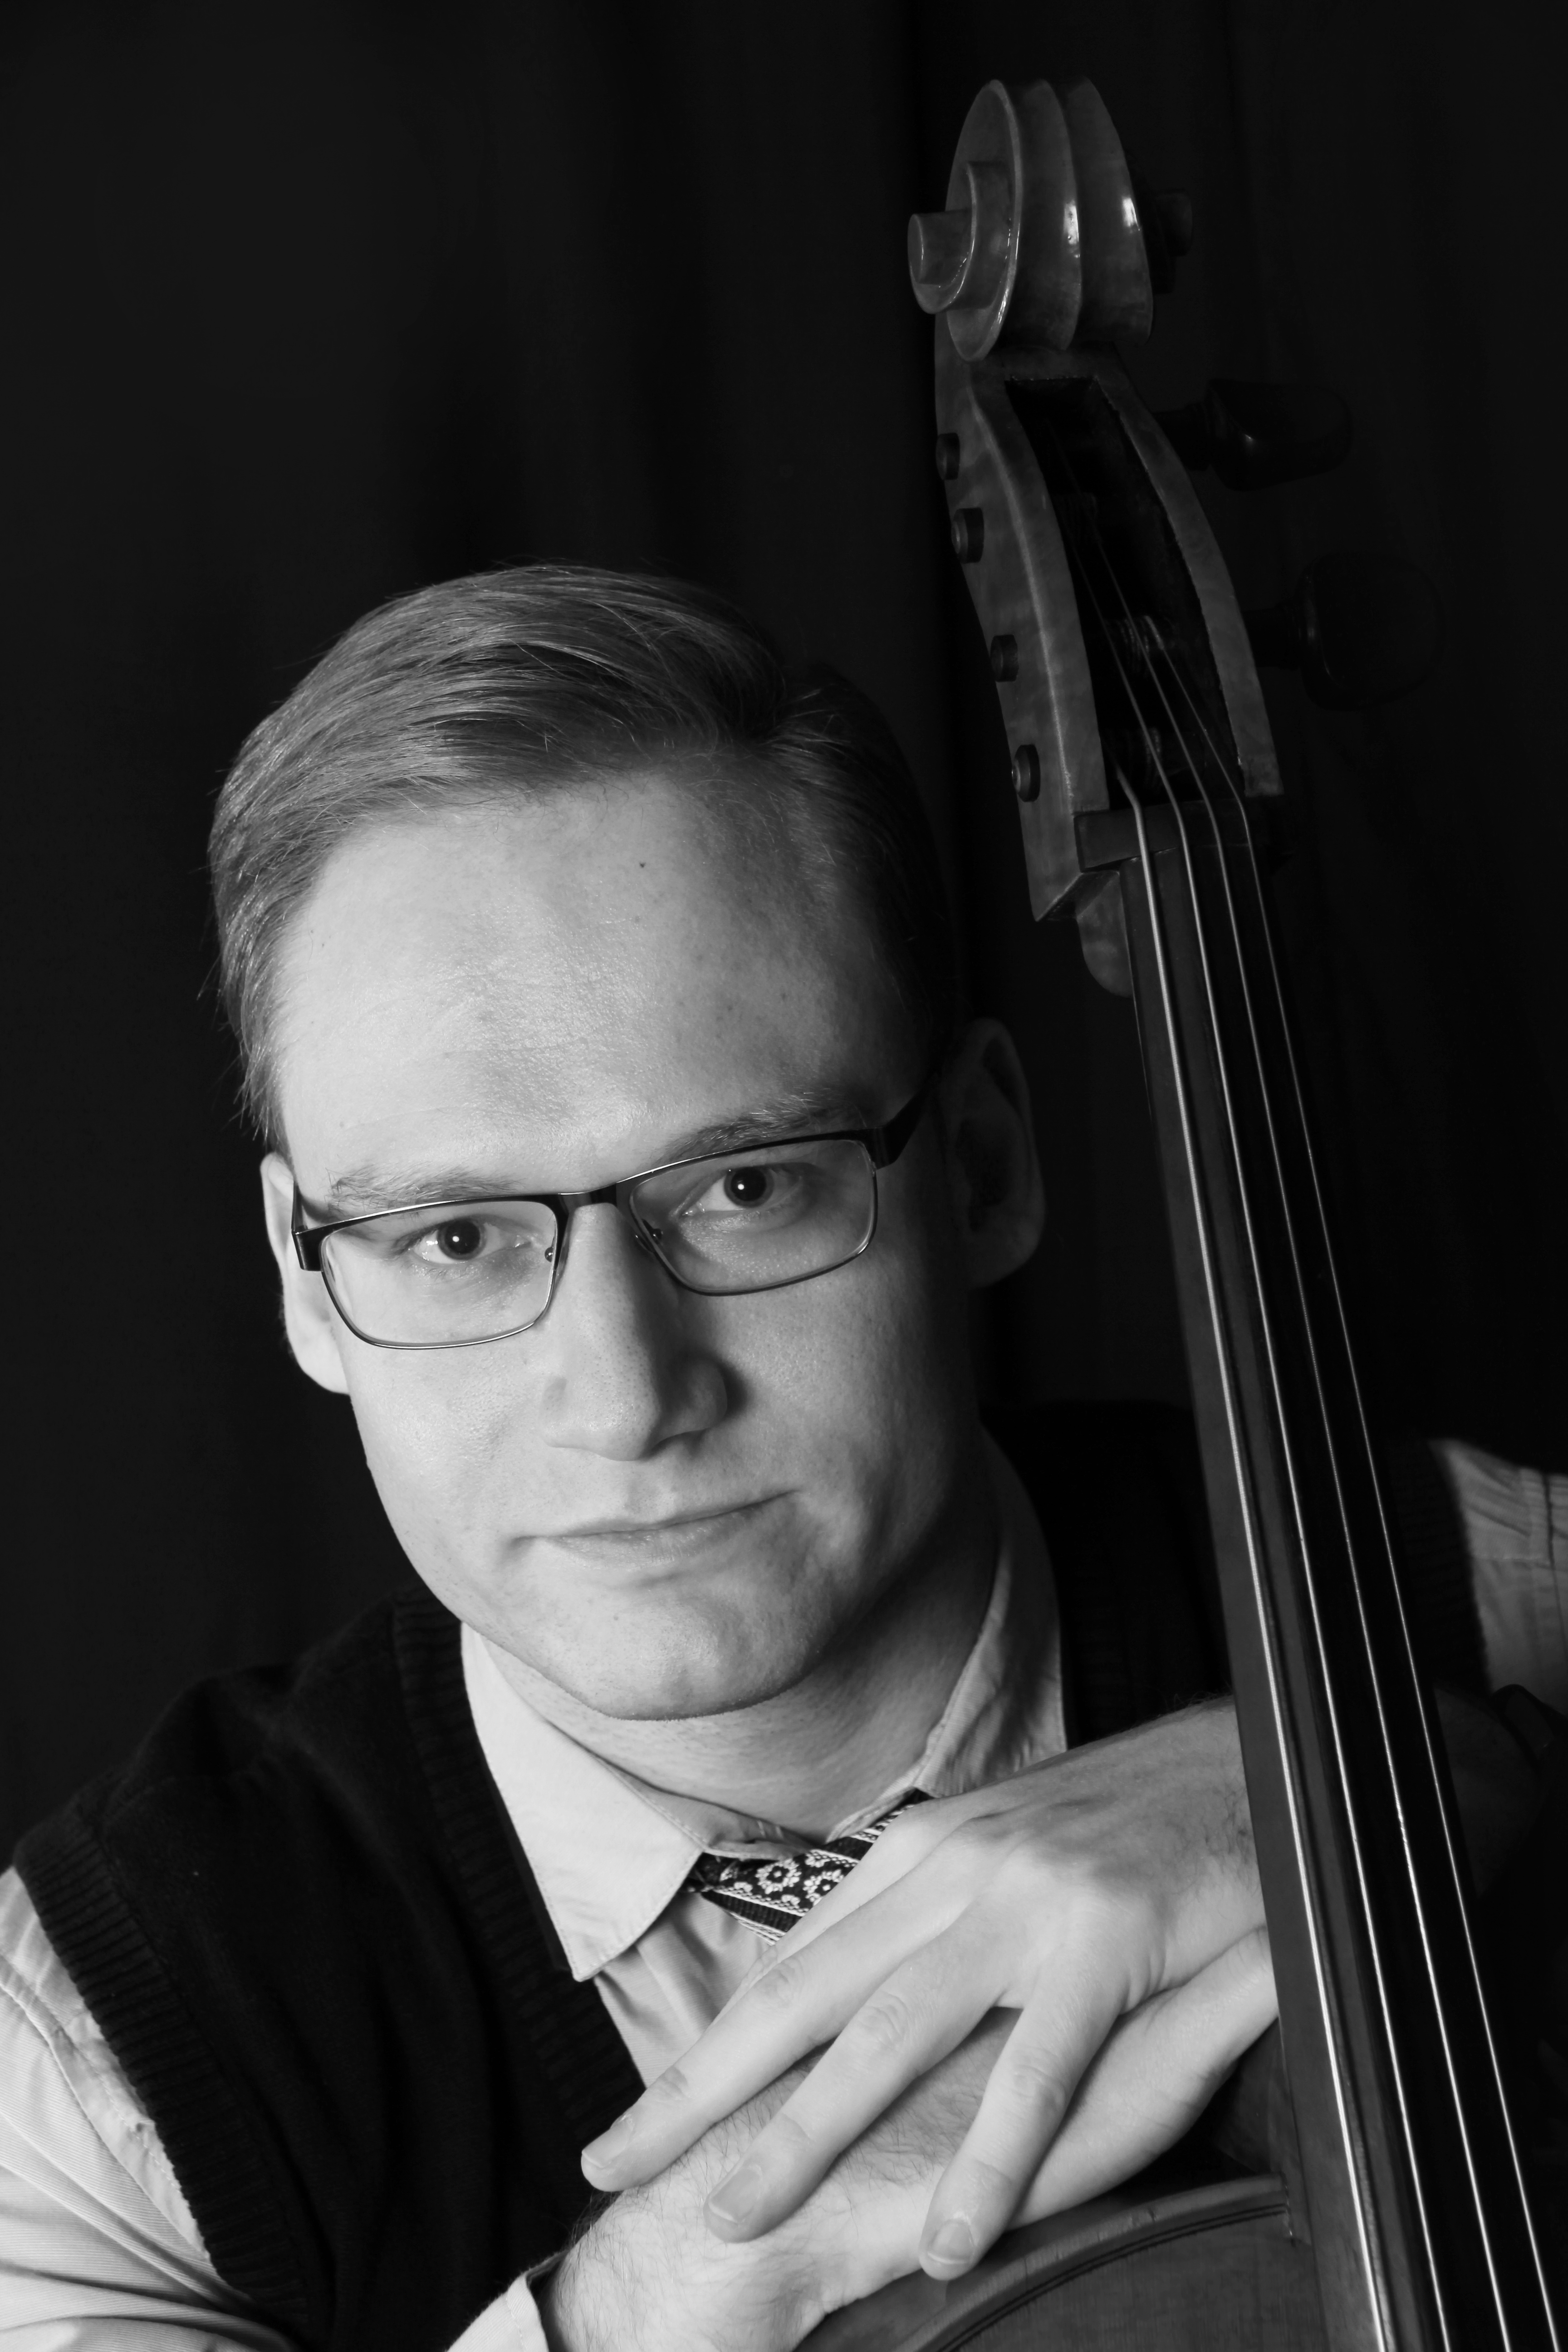
\includegraphics[width=4.6cm]{cello_11a}};
	\end{tikzpicture}
\end{minipage}

\section*{Overview}
I hold a Master's Degree in Space Physics (Cum Laude), which has equipped me with strong research capabilities and proficiency in mathematical analysis and modeling. Transitioning from academia, I gained approximately 3.5 years of experience as a Data Scientist at Matogen Applied Insights. There, I developed solutions such as a Portfolio Performance Monitor and Credit Loss Model for a telecommunications company, a PowerBI dashboard for monitoring agricultural nutrient distributions, and an AI model to predict grape harvesting dates.

To broaden my skillset, I completed a HyperionDev Bootcamp, mastering several programming languages including HTML, CSS, JavaScript, the MERN stack, and Java. This experience enhanced my understanding of full-stack web development and effective database management. Upon completion, I served as a Coding Mentor from July 2024 to the present time.

In summary, I have a strong scientific background, a deep interest in programming, and a naturally curious nature. While I can navigate Windows environments, I prefer working with Linux systems.
\section*{Languages}
\begin{itemize}
	\item \textsc{Afrikaans}: Mother Tongue
	\item \textsc{English}: Fluent, Level 5 TEFL Certification
\end{itemize}

\section*{Education and Training}
\renewcommand{\arraystretch}{1.1}
\begin{tabularx}{\textwidth}{r l X}
	\textbf{2024/07--2025/03} & \multicolumn{2}{| l}{\textbf{\href{https://www.hyperiondev.com/}{HyperionDev}} Code Reviewer \& Student Mentor} \\
	& \multicolumn{1}{| l}{\textbullet} & As a Coding Mentor, I evaluated students' coding submissions for tasks and provided constructive feedback to enhance the quality, efficiency, and styling of their code. Additionally, I conducted live sessions to provide personalised guidance, helping students effectively tackle specific tasks and develop their programming skills. \\
	& \multicolumn{1}{| l}{\textbullet} & Acted as an SME to refactor \href{https://github.com/HenriBranken/AcademicPortfolio/blob/main/06-010-1\_React\%20\textendash\%20Testing\%20a\%20React\%20App.pdf}{\textbf{task contents}} for course syllabi.\\
	& \multicolumn{1}{|l}{\textbullet} & Conducted an \href{https://github.com/HenriBranken/AcademicPortfolio/blob/main/Academic\%20Onboarding\%20Session.pdf}{\textbf{onboarding session}} for newly-enrolled students on the \href{https://livestorm.co/}{\textbf{LiveStorm}} platform. \\
	& \multicolumn{1}{|l}{\textbullet} & Please see my full Academic Portfolio \href{https://github.com/HenriBranken/AcademicPortfolio?tab=readme-ov-file\#academic-portfolio}{\textbf{here}}. \\
	
	& & \\
	
	\textbf{2023/01--2023/09} & \multicolumn{1}{| l}{\textbullet} & 
	\textbf{\href{https://www.hyperiondev.com/bootcamps/immersive/full-stack-web-and-software-engineer/}{HyperionDev Full Stack Web \& Software Engineer Bootcamp}}\\
	& \multicolumn{1}{| l}{\textbullet} & HyperionDev is accredited with the \textbf{\href{https://www.mict.org.za/}{MICT Seta}} (ACC/2017/05/0005). This course bears \textbf{30 Credits}, aligned to an \textbf{NQF Level 5 Qualification}. \\
	& \multicolumn{1}{| l}{\textbullet} & Please click on this \href{https://www.hyperiondev.com/portfolio/79331/}{\textbf{link}} to view my entire HyperionDev Profile.\\
	& \multicolumn{1}{| l}{\textbullet} & I received a \href{https://www.facebook.com/henri.branken.9/posts/pfbid02gUh1H3ovPTfn4TLrr3ZYFWzhcEyuDte2xsZTLbPjHiNZStTRPEArNnius6T5Bj5rl}{\textbf{``Student of the Month'' Award}} for my commitment to excellence and continuous improvement.\\
	& \multicolumn{1}{| l}{\textbullet} & Expand the \textbf{``January 2023 -- September 2023''} section of this \href{https://henribranken.github.io/MyCV/}{link} to view some Git Repos I created during this course.\\
	& & \\	
	\textbf{2022/08--2022/12} & \multicolumn{1}{| l}{\textbullet} &
	\textbf{\href{https://www.theteflacademy.com/za/}{Qualify Level 5 Diploma in Teaching English as a Foreign Language (The TEFL Academy)}} \\
	& \multicolumn{1}{| l}{\textbullet} & Classroom TEFL Course Certificate (20 Hours) \\
	& \multicolumn{1}{| l}{\textbullet} & TEFL, Teaching Business English (30 Hours) \\
	& \multicolumn{1}{| l}{\textbullet} & The completion of my own \href{https://drive.google.com/file/d/1tkuLPdXlgsDundxbjZLjyl6aZhKUqDid/view?usp=sharing}{\textbf{Japanese Language Studies book}}, which took 4+ years. Without a doubt, this is the project I’m most proud of! \\
	
	& & \\
	
	\textbf{2019--2022/07} & \multicolumn{2}{| X}{\textbf{Data Scientist at \href{https://ai.matogen.com/}{Matogen Applied Insights}}} \\
	& & \\
	
	\textbf{2018} & \multicolumn{1}{| l}{\textbullet} & Completed Online Courses at \textbf{\href{https://www.udemy.com/}{Udemy}} and \textbf{\href{https://www.datacamp.com/}{DataCamp}} with a strong focus on \textbf{Python Data Science and Linux Essentials}. \\
	& \multicolumn{1}{| l}{\textbullet} & Attended \textbf{\href{https://2018.za.pycon.org/}{PyConZA 2018}} in Johannesburg.\\
	
	& & \\
	
	\textbf{2017} & \multicolumn{1}{| l}{\textbullet} &
	Internship at the \href{https://natural-sciences.nwu.ac.za/space-research}{\textbf{Centre for Space Research, Potchefstroom}} \\
	& \multicolumn{1}{| l}{\textbullet} & Completed the \textbf{`Data Science with Python' Track} on \href{https://www.datacamp.com/}{\textbf{DataCamp}} (\href{https://www.datacamp.com/Certificate\#13,897}{\textbf{Certificate Number \#13,897}}). \\
	& \multicolumn{1}{| l}{\textbullet} & Completed the 2017 \textbf{\href{https://adventofcode.com/}{Advent of Code}} challenges. My Python solutions may be viewed in this \href{https://github.com/HenriBranken/Advent_of_Code_2017_python_3}{\textbf{repo.}} \\
	& & \\
	
	\textbf{2014--2016} & \multicolumn{2}{| X}{\textbf{Master of Science in \textsc{Space Physics}, \href{https://www.nwu.ac.za/}{North-West University}, Potchefstroom}}\\
	& \multicolumn{2}{| X}{\textsc{Dissertation:} \href{https://repository.nwu.ac.za/handle/10394/25063}{\textit{\textbf{Weighing dark matter in brightest cluster galaxies}}}}\\
	& \multicolumn{2}{| X}{\textsc{Supervisor:} Prof. Ilani Loubser} \\
	& \multicolumn{2}{| X}{\textsc{Avg. Score:} 85\%, \textit{Cum Laude}} \\
	& \multicolumn{2}{| X}{Awarded as the top achiever on Master’s level in the Centre for Space Research (for the year 2016).} \\
	& \multicolumn{2}{| X}{\href{https://github.com/HenriBranken/Henri_Branken_Certification/blob/master/tertiary/full_university_academic_record.pdf}{\textbf{Academic Transcript}}} \\
	& & \\

	\textbf{2013} & \multicolumn{2}{| X}{\textbf{Honours Bachelor of Science in \textsc{Physics}, \href{https://www.nwu.ac.za/}{North-West University}, Potchefstroom}}\\
	& \multicolumn{2}{| X}{\textsc{Avg. Score:} 92\%, \textit{Cum Laude}}\\
	& \multicolumn{2}{| X}{Awarded as the Top Achiever in Honours in Physics.}\\
	& & \\

	\textbf{2010--2012} & \multicolumn{2}{| X}{\textbf{Bachelor of Science in \textsc{Physical and Chemical Sciences}, \href{https://www.nwu.ac.za/}{North-West University}, Potchefstroom}} \\
 	& \multicolumn{2}{| X}{Majored in \textbf{Physics and Applied Mathematics}} \\
 	& \multicolumn{2}{| X}{\textsc{3rd Year Avg. Score:} 95\%, \textit{Cum Laude}} \\
 	& \multicolumn{1}{| l}{\textbullet} & Awarded as the top achiever in the 1\textsuperscript{st}, 2\textsuperscript{nd}, and 3\textsuperscript{rd} years of the Physics curriculum.\\
	& \multicolumn{1}{| l}{\textbullet} & Awarded as the top student in the Faculty of Natural Sciences for the 1\textsuperscript{st} and 3\textsuperscript{rd} years of study.\\
	& \multicolumn{1}{| l}{\textbullet} & Supplemental Instruction Leader for the 2011 Term in Mathematics (1\textsuperscript{st} year level).\\
	& & \\

	\textbf{2009} & \multicolumn{2}{| X}{\textbf{Matriculated with 8 distinctions from St. Andrew’s Private School, Welkom}}\\
	& \multicolumn{2}{| X}{\textbf{Avg. Score:} 89\%, \textit{With Distinction}}\\
\end{tabularx}

\begin{center}
\tikz[mindmap, text=white, grow cyclic, concept color=burnt, font=\Large\bfseries,
root concept/.append style={
},
level 1 concept/.append style={
	sibling angle=90,
	level distance=6cm,
	every child/.style={concept color=teal, font=\bfseries}
},
level 2 concept/.append style={
	sibling angle=45,
	level distance=3cm,
	every child/.style={concept color=tealshade, text=black}
}]
\node [concept] {Henri's Skills}
child {node [concept] {Full-Stack \\ Web Dev}
	child {node [concept] {PHP}}
	child {node [concept] {Java}}
	child {node [concept] {jQuery}}
	child {node [concept] {MERN}}
	child {node [concept] {HTML, CSS, \\ JavaScript}}
}
child {node [concept] {Data Science}
	child {node [concept] {EDA, Data Wrangling}}
	child {node [concept] {PowerBI, Tableau}}
	child {node [concept] {Linux, BASH}}
	child {node [concept] {Git CLI, GitHub}}
	child {node [concept] {Pandas, NumPy, SciPy}}
	child {node [concept] {DataBricks, \\ SnowFlake, SQL, PySpark}}
	child {node [concept] {Python, \\ Jupyter Notebook}}
}
child {node [concept] {Research}
	child {node [concept] {\LaTeX}}
	child {node [concept] {TikZ}}
	child {node [concept] {Maths}}
	child {node [concept] {Physics, Astrophysics}}
	child {node [concept] {LibreOffice Suite}}
	child {node [concept] {ChatGPT}}
}
child {node [concept] {Teaching}
	child {node [concept] {Qualify \\ Level 5 \\ Diploma}}
	child {node [concept] {Teaching \\ Business \\ English}}
	child {node [concept] {Code Reviewer}}
	child {node [concept] {Coding Mentor}}
};
\end{center}

\section*{References}
	\begin{tabularx}{\textwidth}{l X}
	\textbf{Seraaj De Villiers} & HyperionDev \\
	& \faEnvelope \quad \href{mailto:seraajd@hyperiondev.com}{\textbf{seraajd@hyperiondev.com}} \\[0.1cm]
	
	\textbf{Prof. Christo Venter} & North-West University \\
	& \faEnvelope \quad \href{mailto:christo.venter@nwu.ac.za}{\textbf{christo.venter@nwu.ac.za}} \\[0.1cm]
	
	\textbf{Mr. Jacobus Eksteen} & CEO, Matogen Applied Insights \\
	& \faEnvelope \quad \href{mailto:jacobus.eksteen@ai.matogen.com}{\textbf{jacobus.eksteen@ai.matogen.com}} \\[0.1cm]
	
	\textbf{Mr. Bayan Dekker} & Former CEO, BluNova\\
	& \faEnvelope \quad \href{mailto:bayand@versuro.com}{\textbf{bayand@versuro.com}} \\[0.1cm]
	
	\textbf{Ms. Tina Marx} & Data Architect, Matogen Applied Insights\\
	& \faEnvelope \quad \href{mailto:tina.marx@ai.matogen.com}{\textbf{tina.marx@ai.matogen.com}} \\[0.1cm]
\end{tabularx}
	
\end{document}